\documentclass[UTF8,a4paper,11 pt]{ctexart}%字符标准,纸张,字体大小,文档类型,自行打印11pt,单位打印12pt
\usepackage{mathtools,amssymb,array,amsthm,amsmath}%数学宏包
\usepackage{geometry,ulem,graphicx,longtable,caption2,cite,fancyhdr,multicol,color}%通用宏包
\geometry{a4paper,left=1.5cm, right=1.5cm, top=2.6cm, bottom=3cm}%页面布局
\usepackage{siunitx,xfp,empheq,unicode-math}
\sisetup{
	separate-uncertainty = true,
	inter-unit-product = \ensuremath{{}\cdot{}}
}%单位及预设
\usepackage{chemfig,mhchem}%化学宏包
\newcommand\dif{\mathop{}\!\mathrm{d}}%定义微分算子
\newcommand\eu{\mathrm{e}}%定义自然常数
%\renewcommand\bar{\overline}
%\renewcommand\vec{\overrightarrow}
\everymath{\displaystyle}%行间公式
\usepackage{xeCJK,wrapfig}
\usepackage[hidelinks]{hyperref}
\xeCJKsetup{
	CJKecglue={\:}
}
\AtBeginDocument{
	\let\mathbb\relax
	\DeclareMathAlphabet{\mathbb}{U}{msb}{m}{n}
}
\usetikzlibrary{decorations.pathmorphing,patterns,fadings}
\usetikzlibrary {patterns.meta}
\setlength{\lineskip}{8pt}
\setlength{\lineskiplimit}{8pt}
\begin{document}
	\setlength{\lineskip}{8pt}
	\setlength{\lineskiplimit}{8pt}
	\pagestyle{fancy}
	\fancyhead[L]{生物简述报告--20220522}%左页眉,section
	\fancyhead[R]{Written By Feizao From Class 5 With \LaTeX}%右页眉,subsection
	%\fancyfoot[L]{Written By Feizao With \LaTeX} %左页脚
	%\fancyfoot[R]{\thepage} %右页脚
	\fancyhead[C]{} %中页脚
	\fancyfoot[C]{\thepage}
	\begin{center}
		\LARGE{\textbf{关于“新冠病毒核酸检测和抗原检测应用的技术原理”的简述报告}}
	\end{center}
	\mbox{\qquad}壬寅年初,疫情又起。核酸检测(常为咽拭子)与抗原检测(常为鼻拭子)便与我们的生活“不可分离”。
	鉴于本学期学习了《普通高中教科书\quad 生物学\quad 选择性必修3\quad 生物技术与工程》,在此浅谈这两项技术的原理。
	\part{核酸检测}
	顾名思义,“核酸检测”检测的即为核酸。新冠病毒的遗传物质为RNA,检测的也就是其RNA吗?

	是也不是。
	
	其本质上,是通过RT(Reverse Transcription, 逆转录)-PCR(Polymerase Chain Reaction, 聚合酶链式反应)技术,
	先将新冠病毒的核酸RNA进行逆转录为cDNA(complementary DNA, 互补脱氧核糖核酸),再使用PCR技术,使这种cDNA进行扩增,
	便于观察。

	当然这一切,都是要先从我们的咽拭子样本中提取出病毒的RNA。
	具体来说,就是在样本中加入蛋白酶,把病毒破坏,让核酸释放出来。
	\\\textbf{RT技术:}

	由于PCR的扩增对象只能是结构更加稳定的DNA,故先进行逆转录,再扩增。

	我们首先利用逆转录酶,以单链RNA为模板逆转录出cDNA的一条链,如图1所示:
	\begin{figure}[htp!]
		\centering
		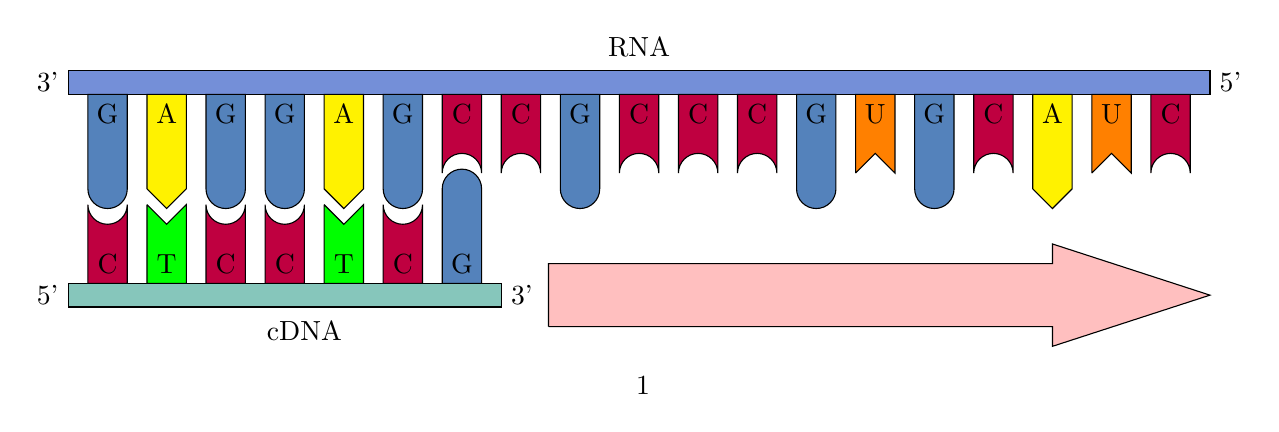
\begin{tikzpicture}
			%GAGGAGCCGCCCGUGCAUC
			\definecolor{qing}{RGB}{134,198,187};
			\definecolor{rna}{RGB}{116,143,216};
			\definecolor{blue}{RGB}{84,130,187};
			\draw[fill=qing] (0,0) rectangle +(5.5,.3);
			\draw[fill=rna] (0,2.7) rectangle +(14.5,.3);
			\draw (0,0)--node[left]{5'}(0,.3);
			\draw (14.5,2.7)--node[right]{5'}+(0,.3);
			\draw (0,2.7)--node[left]{3'}+(0,.3);
			\draw (5.5,0)--node[right]{3'}+(0,.3);
			\foreach \x in {4.75,5.5,7,7.75,8.5,11.5,13.75}{
				\begin{scope}[xshift=\x cm, yshift=2.7 cm]%倒置C
				\draw[fill=purple] (0,-1) -- (0,0)--(.5,0)--(.5,-1)arc (0:180:0.25);
				\node at (.25,-.25) {C};
		\end{scope}
		}
			\foreach \x in {.25,1.75,2.5,4,6.25,9.25,10.75}{
				\begin{scope}[xshift=\x cm, yshift=2.7 cm]%倒置G
					\draw[fill=blue] (0,-1.2) -- (0,0)--(.5,0)--(.5,-1.2)arc (0:-180:0.25);
					\node at (.25,-.25) {G};
				\end{scope}
			}
			\foreach \x in {1,3.25,12.25}{
				\begin{scope}[xshift=\x cm, yshift=2.7 cm]%倒置A
					\draw[fill=yellow] (0,-1.2) -- (0,0)--(.5,0)--(.5,-1.2) --(.25,-1.45)--(0,-1.2);
					\node at (.25,-.25) {A};
				\end{scope}
			}
			\foreach \x in {13,10}{
				\begin{scope}[xshift=\x cm, yshift=2.7 cm]%倒置U
					\draw[fill=orange] (0,-1) -- (0,0)--(.5,0)--(.5,-1) --(.25,-.75)--(0,-1);
					\node at (.25,-.25) {U};
				\end{scope}
			}
			\foreach \x in{.25,1.75,2.5,4}{
				\begin{scope}[xshift=\x cm,yshift=0.3cm]%正立C
					\draw[fill=purple] (0,1) -- (0,0)--(.5,0)--(.5,1)arc (0:-180:0.25);
					\node at (.25,.25) {C};
				\end{scope}	
		}
			\foreach \x in {1,3.25}{
				\begin{scope}[xshift=\x cm, yshift=.3 cm]%正立T
					\draw[fill=green] (0,1) -- (0,0)--(.5,0)--(.5,1) --(.25,.75)--(0,1);
					\node at (.25,.25) {T};
				\end{scope}
			}
			\foreach \x in {4.75}{
				\begin{scope}[xshift=\x cm, yshift=.3 cm]%正立G
					\draw[fill=blue] (0,1.2) -- (0,0)--(.5,0)--(.5,1.2)arc (0:180:0.25);
					\node at (.25,.25) {G};
				\end{scope}
			}
			\draw[fill=pink] (6.1,-.25) -- (12.5,-.25)--(12.5,-.5)--(14.5,.15)--(12.5,.8)--(12.5,.55)--(6.1,.55)--(6.1,-.25);
			\node at (9.3,.15) {逆转录酶};
			\node at (3,-.3) {cDNA};
			\node at (7.25,3+.3) {RNA};
			\node at (7.25,-1) {图1};
		\end{tikzpicture}
	\end{figure}\\其结果如图2所示:
	\begin{figure}[htp!]
		\centering
		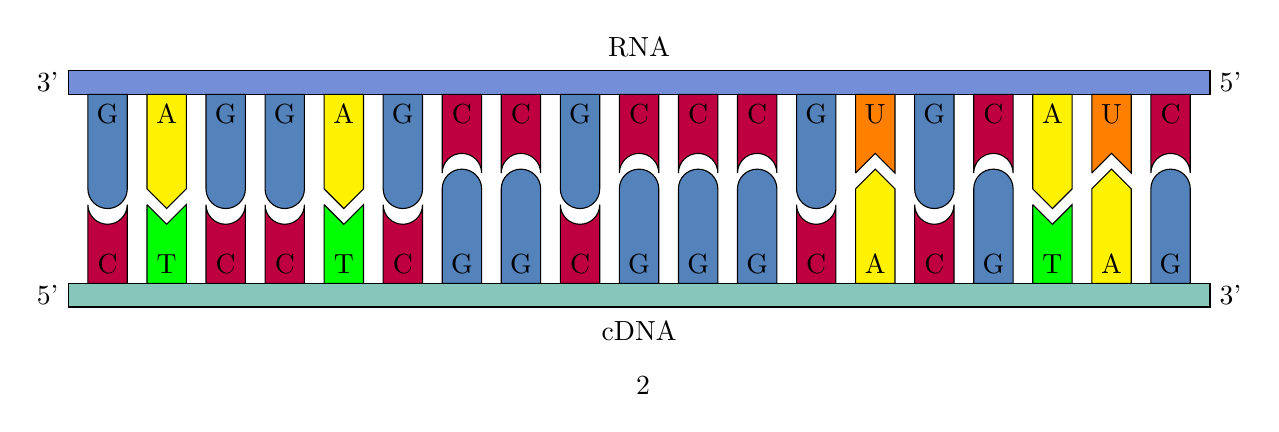
\begin{tikzpicture}
			%GAGGAGCCGCCCGUGCAUC
			%CTCCTCGGCGGGCACGTAG
			\definecolor{qing}{RGB}{134,198,187};
			\definecolor{rna}{RGB}{116,143,216};
			\definecolor{blue}{RGB}{84,130,187};
			\draw[fill=qing] (0,0) rectangle +(14.5,.3);
			\draw[fill=rna] (0,2.7) rectangle +(14.5,.3);
			\draw (0,0)--node[left]{5'}(0,.3);
			\draw (14.5,2.7)--node[right]{5'}+(0,.3);
			\draw (0,2.7)--node[left]{3'}+(0,.3);
			\draw (14.5,0)--node[right]{3'}+(0,.3);
			\foreach \x in {4.75,5.5,7,7.75,8.5,11.5,13.75}{
				\begin{scope}[xshift=\x cm, yshift=2.7 cm]%倒置C
				\draw[fill=purple] (0,-1) -- (0,0)--(.5,0)--(.5,-1)arc (0:180:0.25);
				\node at (.25,-.25) {C};
		\end{scope}
		}
			\foreach \x in {.25,1.75,2.5,4,6.25,9.25,10.75}{
				\begin{scope}[xshift=\x cm, yshift=2.7 cm]%倒置G
					\draw[fill=blue] (0,-1.2) -- (0,0)--(.5,0)--(.5,-1.2)arc (0:-180:0.25);
					\node at (.25,-.25) {G};
				\end{scope}
			}
			\foreach \x in {1,3.25,12.25}{
				\begin{scope}[xshift=\x cm, yshift=2.7 cm]%倒置A
					\draw[fill=yellow] (0,-1.2) -- (0,0)--(.5,0)--(.5,-1.2) --(.25,-1.45)--(0,-1.2);
					\node at (.25,-.25) {A};
				\end{scope}
			}
			\foreach \x in {13,10}{
				\begin{scope}[xshift=\x cm, yshift=2.7 cm]%倒置U
					\draw[fill=orange] (0,-1) -- (0,0)--(.5,0)--(.5,-1) --(.25,-.75)--(0,-1);
					\node at (.25,-.25) {U};
				\end{scope}
			}
			\foreach \x in{.25,1.75,2.5,4,6.25,9.25,10.75}{
				\begin{scope}[xshift=\x cm,yshift=0.3cm]%正立C
					\draw[fill=purple] (0,1) -- (0,0)--(.5,0)--(.5,1)arc (0:-180:0.25);
					\node at (.25,.25) {C};
				\end{scope}	
		}
			\foreach \x in {1,3.25,12.25}{
				\begin{scope}[xshift=\x cm, yshift=.3 cm]%正立T
					\draw[fill=green] (0,1) -- (0,0)--(.5,0)--(.5,1) --(.25,.75)--(0,1);
					\node at (.25,.25) {T};
				\end{scope}
			}
			\foreach \x in {4.75,5.5,7,7.75,8.5,11.5,13.75}{
				\begin{scope}[xshift=\x cm, yshift=.3 cm]%正立G
					\draw[fill=blue] (0,1.2) -- (0,0)--(.5,0)--(.5,1.2)arc (0:180:0.25);
					\node at (.25,.25) {G};
				\end{scope}
			}
			\foreach \x in {13,10}{
				\begin{scope}[xshift=\x cm, yshift=.3 cm]%正立A
					\draw[fill=yellow] (0,1.2) -- (0,0)--(.5,0)--(.5,1.2) --(.25,1.45)--(0,1.2);
					\node at (.25,.25) {A};
				\end{scope}
			}
			\node at (7.25,-.3) {cDNA};
			\node at (7.25,3+.3) {RNA};
			\node at (7.25,-1) {图2};
		\end{tikzpicture}
	\end{figure}

	跟我们的目的是获得稳定的cDNA,图2所示显然不满足要求,
	需要将RNA链替换为与下方cDNA链互补的cDNA链,故利用一种特殊的DNA聚合酶,
	在降解原有的RNA链同时,聚合上脱氧核苷酸并链接其之间的磷酸二酯键,过程如图3所示:
	\begin{figure}[htp!]
		\centering
		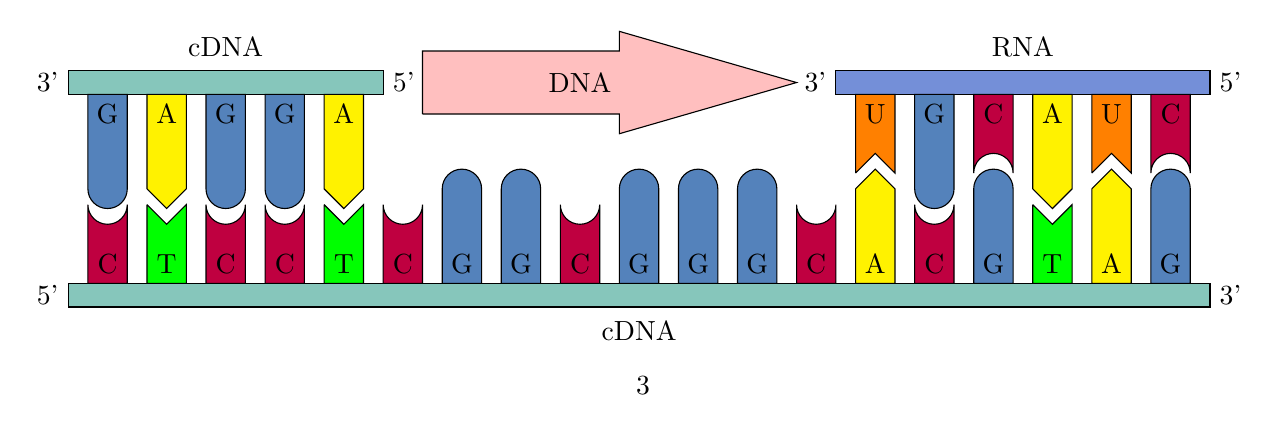
\begin{tikzpicture}
			%GAGGAGCCGCCCGUGCAUC
			\definecolor{qing}{RGB}{134,198,187};
			\definecolor{rna}{RGB}{116,143,216};
			\definecolor{blue}{RGB}{84,130,187};
			\draw[fill=qing] (0,0) rectangle +(14.5,.3);
			\draw[fill=qing] (0,2.7) rectangle +(4,.3);
			\draw[fill=rna] (9.75,2.7) rectangle +(4.75,.3);
			\draw (0,0)--node[left]{5'}(0,.3);
			\draw (0,2.7)--node[left]{3'}+(0,.3);
			\draw (4,2.7)--node[right]{5'}+(0,.3);
			\draw (14.5,2.7)--node[right]{5'}+(0,.3);
			\draw (9.75,2.7)--node[left]{3'}+(0,.3);
			\draw (14.5,0)--node[right]{3'}+(0,.3);
			\foreach \x in {11.5,13.75}{
				\begin{scope}[xshift=\x cm, yshift=2.7 cm]%倒置C
					\draw[fill=purple] (0,-1) -- (0,0)--(.5,0)--(.5,-1)arc (0:180:0.25);
					\node at (.25,-.25) {C};
				\end{scope}
			}
			\foreach \x in {.25,1.75,2.5,10.75}{
				\begin{scope}[xshift=\x cm, yshift=2.7 cm]%倒置G
					\draw[fill=blue] (0,-1.2) -- (0,0)--(.5,0)--(.5,-1.2)arc (0:-180:0.25);
					\node at (.25,-.25) {G};
				\end{scope}
			}
			\foreach \x in {1,3.25,12.25}{
				\begin{scope}[xshift=\x cm, yshift=2.7 cm]%倒置A
					\draw[fill=yellow] (0,-1.2) -- (0,0)--(.5,0)--(.5,-1.2) --(.25,-1.45)--(0,-1.2);
					\node at (.25,-.25) {A};
				\end{scope}
			}
			\foreach \x in {13,10}{
				\begin{scope}[xshift=\x cm, yshift=2.7 cm]%倒置U
					\draw[fill=orange] (0,-1) -- (0,0)--(.5,0)--(.5,-1) --(.25,-.75)--(0,-1);
					\node at (.25,-.25) {U};
				\end{scope}
			}
			\foreach \x in{.25,1.75,2.5,4,6.25,9.25,10.75}{
				\begin{scope}[xshift=\x cm,yshift=0.3cm]%正立C
					\draw[fill=purple] (0,1) -- (0,0)--(.5,0)--(.5,1)arc (0:-180:0.25);
					\node at (.25,.25) {C};
				\end{scope}	
			}
			\foreach \x in {1,3.25,12.25}{
				\begin{scope}[xshift=\x cm, yshift=.3 cm]%正立T
					\draw[fill=green] (0,1) -- (0,0)--(.5,0)--(.5,1) --(.25,.75)--(0,1);
					\node at (.25,.25) {T};
				\end{scope}
			}
			\foreach \x in {4.75,5.5,7,7.75,8.5,11.5,13.75}{
				\begin{scope}[xshift=\x cm, yshift=.3 cm]%正立G
					\draw[fill=blue] (0,1.2) -- (0,0)--(.5,0)--(.5,1.2)arc (0:180:0.25);
					\node at (.25,.25) {G};
				\end{scope}
			}
			\foreach \x in {13,10}{
				\begin{scope}[xshift=\x cm, yshift=.3 cm]%正立A
					\draw[fill=yellow] (0,1.2) -- (0,0)--(.5,0)--(.5,1.2) --(.25,1.45)--(0,1.2);
					\node at (.25,.25) {A};
				\end{scope}
			}
			\begin{scope}[yshift=2.7 cm]
				\draw[fill=pink] (4.5,-.25) -- (7,-.25)--(7,-.5)--(9.25,.15)--(7,.8)--(7,.55)--(4.5,.55)--(4.5,-.25);
				\node at (6.5,.15) {特殊的DNA聚合酶};
			\end{scope}
			\node at (7.25,-.3) {cDNA};
			\node at (12.125,3+.3) {RNA};
			\node at (2,3+.3) {cDNA};
			\node at (7.25,-1) {图3};
		\end{tikzpicture}
	\end{figure}\\
	最终结果如图4:\begin{figure}[htp!]
		\centering
		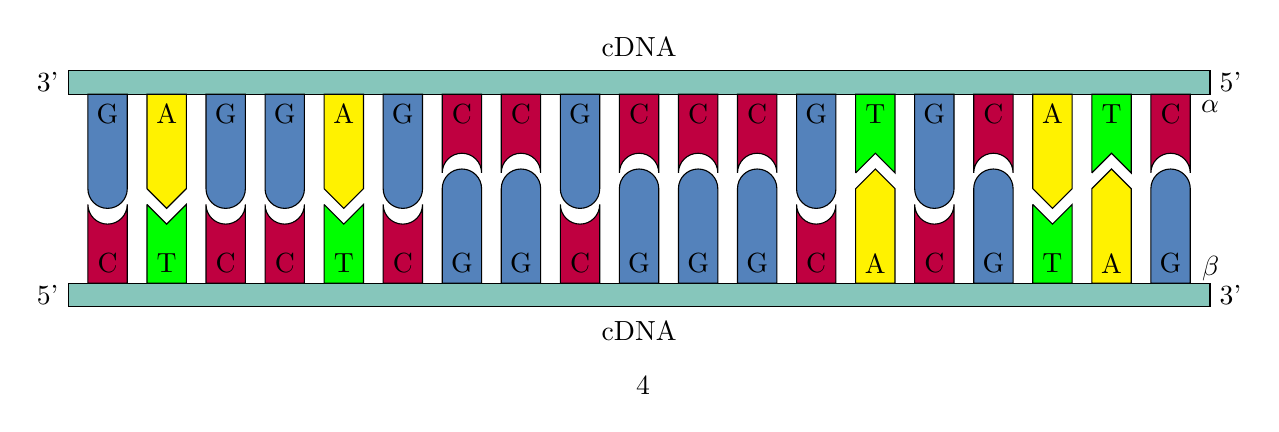
\begin{tikzpicture}
			%GAGGAGCCGCCCGUGCAUC
			\definecolor{qing}{RGB}{134,198,187};
			\definecolor{rna}{RGB}{116,143,216};
			\definecolor{blue}{RGB}{84,130,187};
			\draw[fill=qing] (0,0) rectangle +(14.5,.3);
			\draw[fill=qing] (0,2.7) rectangle +(14.5,.3);
			\draw (0,0)--node[left]{5'}(0,.3);
			\draw (0,2.7)--node[left]{3'}+(0,.3);
			\draw (14.5,2.7)--node[right]{5'}+(0,.3)
			node[below=.25cm]{$\alpha$};
			\draw (14.5,0)node[above=.2cm]{$\beta$}--node[right]{3'}+(0,.3);
			\foreach \x in {4.75,5.5,7,7.75,8.5,11.5,13.75}{
				\begin{scope}[xshift=\x cm, yshift=2.7 cm]%倒置C
					\draw[fill=purple] (0,-1) -- (0,0)--(.5,0)--(.5,-1)arc (0:180:0.25);
					\node at (.25,-.25) {C};
				\end{scope}
			}
			\foreach \x in {.25,1.75,2.5,4,6.25,9.25,10.75}{
				\begin{scope}[xshift=\x cm, yshift=2.7 cm]%倒置G
					\draw[fill=blue] (0,-1.2) -- (0,0)--(.5,0)--(.5,-1.2)arc (0:-180:0.25);
					\node at (.25,-.25) {G};
				\end{scope}
			}
			\foreach \x in {1,3.25,12.25}{
				\begin{scope}[xshift=\x cm, yshift=2.7 cm]%倒置A
					\draw[fill=yellow] (0,-1.2) -- (0,0)--(.5,0)--(.5,-1.2) --(.25,-1.45)--(0,-1.2);
					\node at (.25,-.25) {A};
				\end{scope}
			}
			\foreach \x in {13,10}{
				\begin{scope}[xshift=\x cm, yshift=2.7 cm]%倒置T
					\draw[fill=green] (0,-1) -- (0,0)--(.5,0)--(.5,-1) --(.25,-.75)--(0,-1);
					\node at (.25,-.25) {T};
				\end{scope}
			}
			\foreach \x in{.25,1.75,2.5,4,6.25,9.25,10.75}{
				\begin{scope}[xshift=\x cm,yshift=0.3cm]%正立C
					\draw[fill=purple] (0,1) -- (0,0)--(.5,0)--(.5,1)arc (0:-180:0.25);
					\node at (.25,.25) {C};
				\end{scope}	
			}
			\foreach \x in {1,3.25,12.25}{
				\begin{scope}[xshift=\x cm, yshift=.3 cm]%正立T
					\draw[fill=green] (0,1) -- (0,0)--(.5,0)--(.5,1) --(.25,.75)--(0,1);
					\node at (.25,.25) {T};
				\end{scope}
			}
			\foreach \x in {4.75,5.5,7,7.75,8.5,11.5,13.75}{
				\begin{scope}[xshift=\x cm, yshift=.3 cm]%正立G
					\draw[fill=blue] (0,1.2) -- (0,0)--(.5,0)--(.5,1.2)arc (0:180:0.25);
					\node at (.25,.25) {G};
				\end{scope}
			}
			\foreach \x in {13,10}{
				\begin{scope}[xshift=\x cm, yshift=.3 cm]%正立A
					\draw[fill=yellow] (0,1.2) -- (0,0)--(.5,0)--(.5,1.2) --(.25,1.45)--(0,1.2);
					\node at (.25,.25) {A};
				\end{scope}
			}
			\node at (7.25,-.3) {cDNA};
			\node at (7.25,3+.3) {cDNA};
			\node at (7.25,-1) {图4};
		\end{tikzpicture}
	\end{figure}

	这样,就完成了逆转录即RT技术的全程。
	\\\textbf{PCR技术(荧光):}

	鉴于教科书中对此部分有些许介绍,故不介绍其基本原理,只说明在荧光探针的辅助下的作用原理。

	以$\alpha$链的扩增为例(假设$\beta$链上不含有能与荧光探针
	互补的片段,故略去$\beta$链),如图5所示,引物$\alpha$与3'段结合,
	而荧光探针与中间的某一片段结合:\begin{figure}[htp!]
		\centering
		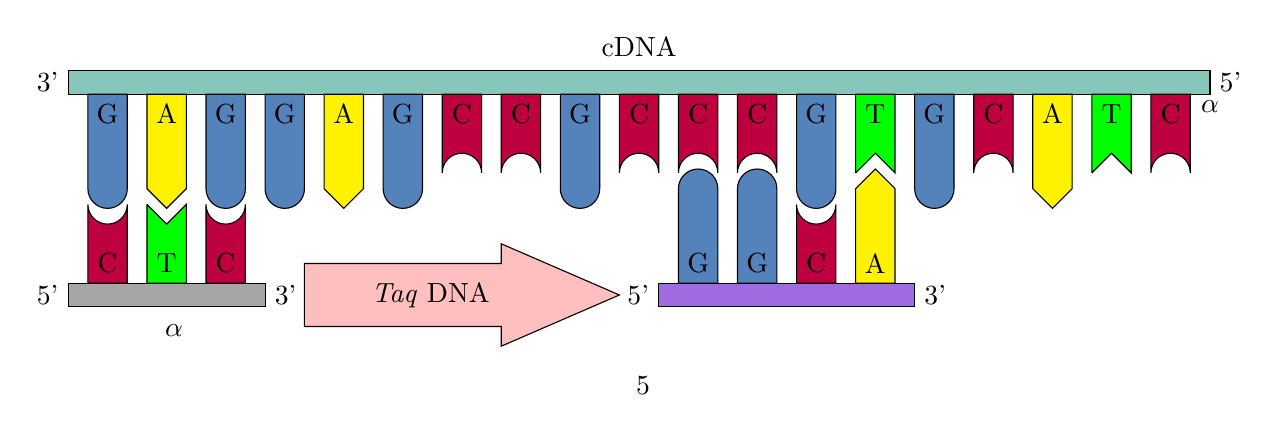
\begin{tikzpicture}
			%GAGGAGCCGCCCGUGCAUC
			\definecolor{qing}{RGB}{134,198,187};
			\definecolor{rna}{RGB}{116,143,216};
			\definecolor{blue}{RGB}{84,130,187};
			\definecolor{grey}{RGB}{166,166,166};
			\definecolor{ying}{RGB}{160,107,224}
			\draw[fill=grey] (0,0) rectangle +(2.5,.3);
			\draw[fill=qing] (0,2.7) rectangle +(14.5,.3);
			\draw[fill=ying] (7.5,0) rectangle (10.75,.3);
			\draw (0,2.7)--node[left]{3'}+(0,.3);
			\draw (14.5,2.7)--node[right]{5'}+(0,.3)node[below=.25cm]{$\alpha$};
			\draw (0,0)--node[left]{5'}(0,.3);
			\draw (2.5,0)--node[right]{3'}+(0,.3);
			\draw (7.5,0)--node[left]{5'}+(0,.3);
			\draw (10.75,0)--node[right]{3'}+(0,.3);
			;
			\foreach \x in {4.75,5.5,7,7.75,8.5,11.5,13.75}{
				\begin{scope}[xshift=\x cm, yshift=2.7 cm]%倒置C
					\draw[fill=purple] (0,-1) -- (0,0)--(.5,0)--(.5,-1)arc (0:180:0.25);
					\node at (.25,-.25) {C};
				\end{scope}
			}
			\foreach \x in {.25,1.75,2.5,4,6.25,9.25,10.75}{
				\begin{scope}[xshift=\x cm, yshift=2.7 cm]%倒置G
					\draw[fill=blue] (0,-1.2) -- (0,0)--(.5,0)--(.5,-1.2)arc (0:-180:0.25);
					\node at (.25,-.25) {G};
				\end{scope}
			}
			\foreach \x in {1,3.25,12.25}{
				\begin{scope}[xshift=\x cm, yshift=2.7 cm]%倒置A
					\draw[fill=yellow] (0,-1.2) -- (0,0)--(.5,0)--(.5,-1.2) --(.25,-1.45)--(0,-1.2);
					\node at (.25,-.25) {A};
				\end{scope}
			}
			\foreach \x in {13,10}{
				\begin{scope}[xshift=\x cm, yshift=2.7 cm]%倒置T
					\draw[fill=green] (0,-1) -- (0,0)--(.5,0)--(.5,-1) --(.25,-.75)--(0,-1);
					\node at (.25,-.25) {T};
				\end{scope}
			}
			\foreach \x in{.25,1.75,9.25}{
				\begin{scope}[xshift=\x cm,yshift=0.3cm]%正立C
					\draw[fill=purple] (0,1) -- (0,0)--(.5,0)--(.5,1)arc (0:-180:0.25);
					\node at (.25,.25) {C};
				\end{scope}	
			}
			\foreach \x in {1}{
				\begin{scope}[xshift=\x cm, yshift=.3 cm]%正立T
					\draw[fill=green] (0,1) -- (0,0)--(.5,0)--(.5,1) --(.25,.75)--(0,1);
					\node at (.25,.25) {T};
				\end{scope}
			}
			\foreach \x in {7.75,8.5}{
				\begin{scope}[xshift=\x cm, yshift=.3 cm]%正立G
					\draw[fill=blue] (0,1.2) -- (0,0)--(.5,0)--(.5,1.2)arc (0:180:0.25);
					\node at (.25,.25) {G};
				\end{scope}
			}
			\foreach \x in {10}{
				\begin{scope}[xshift=\x cm, yshift=.3 cm]%正立A
					\draw[fill=yellow] (0,1.2) -- (0,0)--(.5,0)--(.5,1.2) --(.25,1.45)--(0,1.2);
					\node at (.25,.25) {A};
				\end{scope}
			}
			\begin{scope}[yshift=0 cm]
				\draw[fill=pink] (3,-.25) -- (5.5,-.25)--(5.5,-.5)--(7,.15)--(5.5,.8)--(5.5,.55)--(3,.55)--(3,-.25);
				\node at (4.75,.15) {\textit{Taq} DNA聚合酶};
			\end{scope}
			\node at (1.25,-.3) {引物$ \alpha $};
			\node at (18.25/2,-.3) {荧光探针};
			\node at (7.25,3+.3) {cDNA};
			\node at (7.25,-1) {图5};
		\end{tikzpicture}
	\end{figure}

	随着\textit{Taq} 聚合酶的推进,荧光探针逐渐被破坏,发出荧光,
	PCR检测仪接接收到荧光信号,并记录这个的数目。

	假设最开始有$N$个双链cDNA,则显然第$n$个循环后,
	理论产生的荧光次数\begin{align*}
		t_n&=N\cdot2^n\cdot\dfrac{1}{2}
		\\&=N\cdot2^{n-1}.
	\end{align*}
	
	一般取$35\sim 40$个循环后的结果,
	若此时$t_n$的特别的大,则认为是阳性,否则为阴性。

	至此,核酸检测的所有步骤结束。
	\part{抗原检测}

	下面介绍鼻拭子即抗原检测的原理。

	从病毒的结构上讲,其表面有多种蛋白,如S蛋白、M蛋白、核衣壳蛋白等。
	为了检测的高效性,一般取用最多的核衣壳蛋白,其在病毒侵染受感染者的
	呼吸道上皮细胞时,便会产生这种蛋白。

	我们将鼻拭子塞入鼻腔,转动的过程中就很好的接触了上皮细胞,并使得病毒
	附着在了鼻拭子的棉头上。随后,我们将鼻拭子棉头放入缓冲液中,挤压、搅拌,使得
	抗原(核衣壳蛋白)释放于溶液中,随后便进入关键步骤:试剂盒对缓冲液的检测。

	首先我们要先了解试剂盒的结构。其表面有样品孔(滴入缓冲液的孔)与检测线(Test Line即T)和对照线(Control Line即C)。
	而其内部结构如图6所示:
	\begin{figure}[htp!]
		\centering
		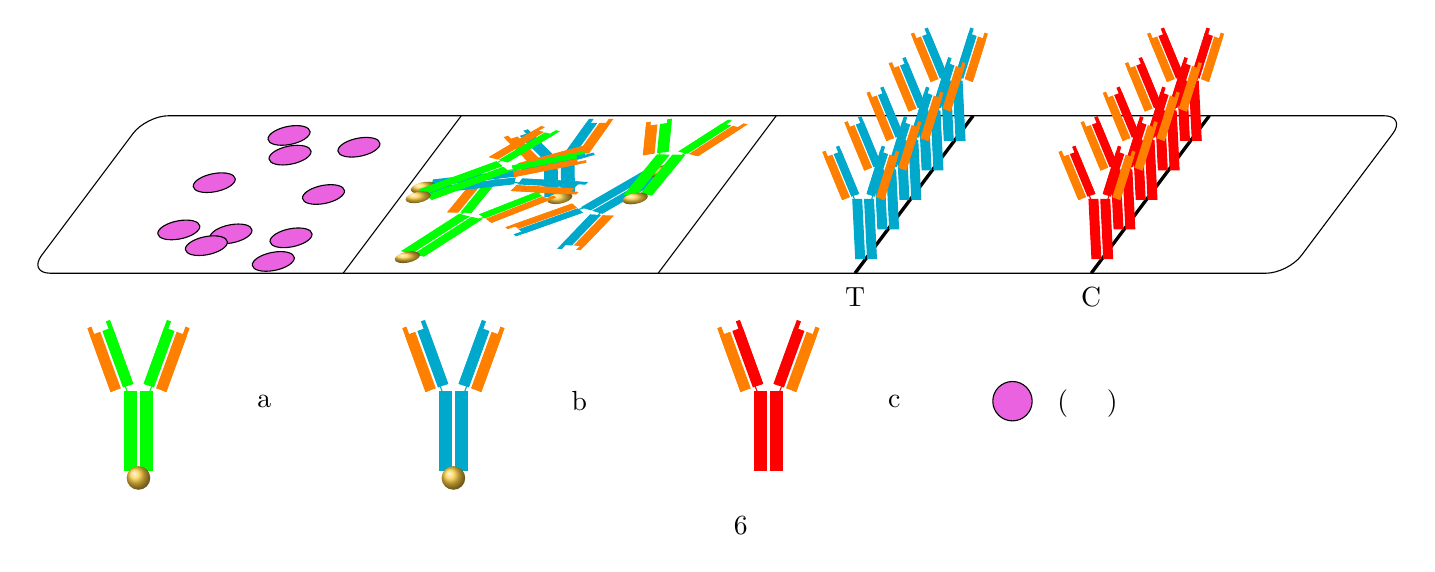
\begin{tikzpicture}
			\definecolor{pink}{RGB}{234,98,223};
			\definecolor{blue}{RGB}{0,169,204};
			\definecolor{gold}{RGB}{250,203,61};
			\begin{scope}[xslant=0.75,yscale=0.5]
				\draw[rounded corners=8pt] (0,0) rectangle +(16,4);
				\foreach \x in{4,8}
				\draw (\x,0)--(\x,4);
				\foreach \x in{10.5,13.5}
				\draw[very thick] (\x,0)--(\x,4);
				\draw[fill=pink] (2.2,3) circle (0.25);
				\draw[fill=pink] (1.5,2.3) circle (0.25);
				\draw[fill=pink] (3,2) circle (0.25);
				\draw[fill=pink] (2,3.5) circle (0.25);
				\draw[fill=pink] (3,3.2) circle (0.25);
				\draw[fill=pink] (2.2,3-2) circle (0.25);
				\draw[fill=pink] (1.5,2.3-1.2) circle (0.25);
				\draw[fill=pink] (3,2-1.7) circle (0.25);
				\draw[fill=pink] (2,3.5-2.8) circle (0.25);
				\draw[fill=pink] (3,3.4-2.5) circle (0.25);
				\begin{scope}[xshift=6cm,yshift=2 cm]%新抗
					\begin{scope}[rotate=21]
						\begin{scope}[xshift=0.025 cm];
							\draw[color=blue, fill=blue] (0,0)rectangle+(.15,1);
							\draw[blue] (0.1,.95)--(.175,1.15);
							\begin{scope}[xshift=.05 cm, yshift=1.1 cm]
								\draw[color=blue, fill=blue, rotate=-20]
								(0,0)rectangle +(.125,.75);
								\draw[color=blue, fill=blue, rotate=-20]
								(0,0)rectangle +(.125/3,.85);
							\end{scope}
							\begin{scope}[xshift=.325 cm, yshift=1 cm]
								\draw[color=orange, fill=orange, rotate=-20]
								(0,0)rectangle +(-.125,.75);
								\draw[color=orange, fill=orange, rotate=-20]
								(0,0)rectangle +(-.125/3,.85);
							\end{scope}
						\end{scope}
						\begin{scope}[xshift=-0.025 cm, xscale=-1];
							\draw[color=blue, fill=blue] (0,0)rectangle+(.15,1);
							\draw[blue] (0.1,.95)--(.175,1.15);
							\begin{scope}[xshift=.05 cm, yshift=1.1 cm]
								\draw[color=blue, fill=blue, rotate=-20]
								(0,0)rectangle +(.125,.75);
								\draw[color=blue, fill=blue, rotate=-20]
								(0,0)rectangle +(.125/3,.85);
							\end{scope}
							\begin{scope}[xshift=.325 cm, yshift=1 cm]
								\draw[color=orange, fill=orange, rotate=-20]
								(0,0)rectangle +(-.125,.75);
								\draw[color=orange, fill=orange, rotate=-20]
								(0,0)rectangle +(-.125/3,.85);
							\end{scope}
						\end{scope}
						\shade [ball color=gold] (0,-.1) circle (0.15);
					\end{scope}
				\end{scope}
				\begin{scope}[xshift=4.7cm,yshift=.5 cm]%控
					\begin{scope}[rotate=-22]
						\begin{scope}[xshift=0.025 cm];
							\draw[color=green, fill=green] (0,0)rectangle+(.15,1);
							\draw[green] (0.1,.95)--(.175,1.15);
							\begin{scope}[xshift=.05 cm, yshift=1.1 cm]
								\draw[color=green, fill=green, rotate=-20]
								(0,0)rectangle +(.125,.75);
								\draw[color=green, fill=green, rotate=-20]
								(0,0)rectangle +(.125/3,.85);
							\end{scope}
							\begin{scope}[xshift=.325 cm, yshift=1 cm]
								\draw[color=orange, fill=orange, rotate=-20]
								(0,0)rectangle +(-.125,.75);
								\draw[color=orange, fill=orange, rotate=-20]
								(0,0)rectangle +(-.125/3,.85);
							\end{scope}
						\end{scope}
						\begin{scope}[xshift=-0.025 cm, xscale=-1];
							\draw[color=green, fill=green] (0,0)rectangle+(.15,1);
							\draw[green] (0.1,.95)--(.175,1.15);
							\begin{scope}[xshift=.05 cm, yshift=1.1 cm]
								\draw[color=green, fill=green, rotate=-20]
								(0,0)rectangle +(.125,.75);
								\draw[color=green, fill=green, rotate=-20]
								(0,0)rectangle +(.125/3,.85);
							\end{scope}
							\begin{scope}[xshift=.325 cm, yshift=1 cm]
								\draw[color=orange, fill=orange, rotate=-20]
								(0,0)rectangle +(-.125,.75);
								\draw[color=orange, fill=orange, rotate=-20]
								(0,0)rectangle +(-.125/3,.85);
							\end{scope}
						\end{scope}
						\shade [ball color=gold] (0,-.1) circle (0.15);
					\end{scope}
				\end{scope}
				\begin{scope}[xshift=7cm,yshift=2.5 cm]%新抗
					\begin{scope}[rotate=154]
						\begin{scope}[xshift=0.025 cm];
							\draw[color=blue, fill=blue] (0,0)rectangle+(.15,1);
							\draw[blue] (0.1,.95)--(.175,1.15);
							\begin{scope}[xshift=.05 cm, yshift=1.1 cm]
								\draw[color=blue, fill=blue, rotate=-20]
								(0,0)rectangle +(.125,.75);
								\draw[color=blue, fill=blue, rotate=-20]
								(0,0)rectangle +(.125/3,.85);
							\end{scope}
							\begin{scope}[xshift=.325 cm, yshift=1 cm]
								\draw[color=orange, fill=orange, rotate=-20]
								(0,0)rectangle +(-.125,.75);
								\draw[color=orange, fill=orange, rotate=-20]
								(0,0)rectangle +(-.125/3,.85);
							\end{scope}
						\end{scope}
						\begin{scope}[xshift=-0.025 cm, xscale=-1];
							\draw[color=blue, fill=blue] (0,0)rectangle+(.15,1);
							\draw[blue] (0.1,.95)--(.175,1.15);
							\begin{scope}[xshift=.05 cm, yshift=1.1 cm]
								\draw[color=blue, fill=blue, rotate=-20]
								(0,0)rectangle +(.125,.75);
								\draw[color=blue, fill=blue, rotate=-20]
								(0,0)rectangle +(.125/3,.85);
							\end{scope}
							\begin{scope}[xshift=.325 cm, yshift=1 cm]
								\draw[color=orange, fill=orange, rotate=-20]
								(0,0)rectangle +(-.125,.75);
								\draw[color=orange, fill=orange, rotate=-20]
								(0,0)rectangle +(-.125/3,.85);
							\end{scope}
						\end{scope}
						\shade [ball color=gold] (0,-.1) circle (0.15);
					\end{scope}
				\end{scope}
				\begin{scope}[xshift=7cm,yshift=2cm]%控
					\begin{scope}[rotate=-2]
						\begin{scope}[xshift=0.025 cm];
							\draw[color=green, fill=green] (0,0)rectangle+(.15,1);
							\draw[green] (0.1,.95)--(.175,1.15);
							\begin{scope}[xshift=.05 cm, yshift=1.1 cm]
								\draw[color=green, fill=green, rotate=-20]
								(0,0)rectangle +(.125,.75);
								\draw[color=green, fill=green, rotate=-20]
								(0,0)rectangle +(.125/3,.85);
							\end{scope}
							\begin{scope}[xshift=.325 cm, yshift=1 cm]
								\draw[color=orange, fill=orange, rotate=-20]
								(0,0)rectangle +(-.125,.75);
								\draw[color=orange, fill=orange, rotate=-20]
								(0,0)rectangle +(-.125/3,.85);
							\end{scope}
						\end{scope}
						\begin{scope}[xshift=-0.025 cm, xscale=-1];
							\draw[color=green, fill=green] (0,0)rectangle+(.15,1);
							\draw[green] (0.1,.95)--(.175,1.15);
							\begin{scope}[xshift=.05 cm, yshift=1.1 cm]
								\draw[color=green, fill=green, rotate=-20]
								(0,0)rectangle +(.125,.75);
								\draw[color=green, fill=green, rotate=-20]
								(0,0)rectangle +(.125/3,.85);
							\end{scope}
							\begin{scope}[xshift=.325 cm, yshift=1 cm]
								\draw[color=orange, fill=orange, rotate=-20]
								(0,0)rectangle +(-.125,.75);
								\draw[color=orange, fill=orange, rotate=-20]
								(0,0)rectangle +(-.125/3,.85);
							\end{scope}
						\end{scope}
						\shade [ball color=gold] (0,-.1) circle (0.15);
					\end{scope}
				\end{scope}
				\begin{scope}[xshift=4.3cm,yshift=2.2 cm]%新抗
					\begin{scope}[rotate=-76]
						\begin{scope}[xshift=0.025 cm];
							\draw[color=blue, fill=blue] (0,0)rectangle+(.15,1);
							\draw[blue] (0.1,.95)--(.175,1.15);
							\begin{scope}[xshift=.05 cm, yshift=1.1 cm]
								\draw[color=blue, fill=blue, rotate=-20]
								(0,0)rectangle +(.125,.75);
								\draw[color=blue, fill=blue, rotate=-20]
								(0,0)rectangle +(.125/3,.85);
							\end{scope}
							\begin{scope}[xshift=.325 cm, yshift=1 cm]
								\draw[color=orange, fill=orange, rotate=-20]
								(0,0)rectangle +(-.125,.75);
								\draw[color=orange, fill=orange, rotate=-20]
								(0,0)rectangle +(-.125/3,.85);
							\end{scope}
						\end{scope}
						\begin{scope}[xshift=-0.025 cm, xscale=-1];
							\draw[color=blue, fill=blue] (0,0)rectangle+(.15,1);
							\draw[blue] (0.1,.95)--(.175,1.15);
							\begin{scope}[xshift=.05 cm, yshift=1.1 cm]
								\draw[color=blue, fill=blue, rotate=-20]
								(0,0)rectangle +(.125,.75);
								\draw[color=blue, fill=blue, rotate=-20]
								(0,0)rectangle +(.125/3,.85);
							\end{scope}
							\begin{scope}[xshift=.325 cm, yshift=1 cm]
								\draw[color=orange, fill=orange, rotate=-20]
								(0,0)rectangle +(-.125,.75);
								\draw[color=orange, fill=orange, rotate=-20]
								(0,0)rectangle +(-.125/3,.85);
							\end{scope}
						\end{scope}
						\shade [ball color=gold] (0,-.1) circle (0.15);
					\end{scope}
				\end{scope}
				\begin{scope}[xshift=4.3cm,yshift=2 cm]%控
					\begin{scope}[rotate=-45]
						\begin{scope}[xshift=0.025 cm];
							\draw[color=green, fill=green] (0,0)rectangle+(.15,1);
							\draw[green] (0.1,.95)--(.175,1.15);
							\begin{scope}[xshift=.05 cm, yshift=1.1 cm]
								\draw[color=green, fill=green, rotate=-20]
								(0,0)rectangle +(.125,.75);
								\draw[color=green, fill=green, rotate=-20]
								(0,0)rectangle +(.125/3,.85);
							\end{scope}
							\begin{scope}[xshift=.325 cm, yshift=1 cm]
								\draw[color=orange, fill=orange, rotate=-20]
								(0,0)rectangle +(-.125,.75);
								\draw[color=orange, fill=orange, rotate=-20]
								(0,0)rectangle +(-.125/3,.85);
							\end{scope}
						\end{scope}
						\begin{scope}[xshift=-0.025 cm, xscale=-1];
							\draw[color=green, fill=green] (0,0)rectangle+(.15,1);
							\draw[green] (0.1,.95)--(.175,1.15);
							\begin{scope}[xshift=.05 cm, yshift=1.1 cm]
								\draw[color=green, fill=green, rotate=-20]
								(0,0)rectangle +(.125,.75);
								\draw[color=green, fill=green, rotate=-20]
								(0,0)rectangle +(.125/3,.85);
							\end{scope}
							\begin{scope}[xshift=.325 cm, yshift=1 cm]
								\draw[color=orange, fill=orange, rotate=-20]
								(0,0)rectangle +(-.125,.75);
								\draw[color=orange, fill=orange, rotate=-20]
								(0,0)rectangle +(-.125/3,.85);
							\end{scope}
						\end{scope}
						\shade [ball color=gold] (0,-.1) circle (0.15);
					\end{scope}
				\end{scope}
				\foreach \x in {4.5,3.5,...,.5}{
					\begin{scope}[scale=0.75,xshift=18cm,yshift=\x cm,xslant=-.4,yscale=2]%抗抗
						\begin{scope}[rotate=0]
							\begin{scope}[xshift=0.025 cm];
								\draw[color=red, fill=red] (0,0)rectangle+(.15,1);
								\draw[red] (0.1,.95)--(.175,1.15);
								\begin{scope}[xshift=.05 cm, yshift=1.1 cm]
									\draw[color=red, fill=red, rotate=-20]
									(0,0)rectangle +(.125,.75);
									\draw[color=red, fill=red, rotate=-20]
									(0,0)rectangle +(.125/3,.85);
								\end{scope}
								\begin{scope}[xshift=.325 cm, yshift=1 cm]
									\draw[color=orange, fill=orange, rotate=-20]
									(0,0)rectangle +(-.125,.75);
									\draw[color=orange, fill=orange, rotate=-20]
									(0,0)rectangle +(-.125/3,.85);
								\end{scope}
							\end{scope}
							\begin{scope}[xshift=-0.025 cm, xscale=-1];
								\draw[color=red, fill=red] (0,0)rectangle+(.15,1);
								\draw[red] (0.1,.95)--(.175,1.15);
								\begin{scope}[xshift=.05 cm, yshift=1.1 cm]
									\draw[color=red, fill=red, rotate=-20]
									(0,0)rectangle +(.125,.75);
									\draw[color=red, fill=red, rotate=-20]
									(0,0)rectangle +(.125/3,.85);
								\end{scope}
								\begin{scope}[xshift=.325 cm, yshift=1 cm]
									\draw[color=orange, fill=orange, rotate=-20]
									(0,0)rectangle +(-.125,.75);
									\draw[color=orange, fill=orange, rotate=-20]
									(0,0)rectangle +(-.125/3,.85);
								\end{scope}
							\end{scope}
						\end{scope}
					\end{scope}	
				}
				%ff
				%dads
				\foreach \x in {4.5,3.5,...,.5}{
					\begin{scope}[scale=0.75,xshift=14cm,yshift=\x cm,xslant=-.4,yscale=2]%抗抗
						\begin{scope}[rotate=0]
							\begin{scope}[xshift=0.025 cm];
								\draw[color=blue, fill=blue] (0,0)rectangle+(.15,1);
								\draw[blue] (0.1,.95)--(.175,1.15);
								\begin{scope}[xshift=.05 cm, yshift=1.1 cm]
									\draw[color=blue, fill=blue, rotate=-20]
									(0,0)rectangle +(.125,.75);
									\draw[color=blue, fill=blue, rotate=-20]
									(0,0)rectangle +(.125/3,.85);
								\end{scope}
								\begin{scope}[xshift=.325 cm, yshift=1 cm]
									\draw[color=orange, fill=orange, rotate=-20]
									(0,0)rectangle +(-.125,.75);
									\draw[color=orange, fill=orange, rotate=-20]
									(0,0)rectangle +(-.125/3,.85);
								\end{scope}
							\end{scope}
							\begin{scope}[xshift=-0.025 cm, xscale=-1];
								\draw[color=blue, fill=blue] (0,0)rectangle+(.15,1);
								\draw[blue] (0.1,.95)--(.175,1.15);
								\begin{scope}[xshift=.05 cm, yshift=1.1 cm]
									\draw[color=blue, fill=blue, rotate=-20]
									(0,0)rectangle +(.125,.75);
									\draw[color=blue, fill=blue, rotate=-20]
									(0,0)rectangle +(.125/3,.85);
								\end{scope}
								\begin{scope}[xshift=.325 cm, yshift=1 cm]
									\draw[color=orange, fill=orange, rotate=-20]
									(0,0)rectangle +(-.125,.75);
									\draw[color=orange, fill=orange, rotate=-20]
									(0,0)rectangle +(-.125/3,.85);
								\end{scope}
							\end{scope}
						\end{scope}
					\end{scope}	
				}
				%dasda
			\end{scope}
			\node at (2,-.3) {样品垫};
			\node at (6,-.3) {聚集垫};
			\node at (10.5,-.3) {T};
			\node at (13.5,-.3) {C};
			\node at (12,-.3) {检测区};
			\draw[fill=pink] (12.5,-1.625) circle (0.25);
			\draw (12.5+.25,-1.65)node[right]{抗原(核衣壳蛋白)};
			\begin{scope}[yshift=0 cm,xshift=.4cm]
				\begin{scope}[xshift=1 cm,yshift=-2.5 cm]%控
					\node at (1.5,7/8) {抗体a};				\begin{scope}[rotate=0]
						\begin{scope}[xshift=0.025 cm];
							\draw[color=green, fill=green] (0,0)rectangle+(.15,1);
							\draw[green] (0.1,.95)--(.175,1.15);
							\begin{scope}[xshift=.05 cm, yshift=1.1 cm]
								\draw[color=green, fill=green, rotate=-20]
								(0,0)rectangle +(.125,.75);
								\draw[color=green, fill=green, rotate=-20]
								(0,0)rectangle +(.125/3,.85);
							\end{scope}
							\begin{scope}[xshift=.325 cm, yshift=1 cm]
								\draw[color=orange, fill=orange, rotate=-20]
								(0,0)rectangle +(-.125,.75);
								\draw[color=orange, fill=orange, rotate=-20]
								(0,0)rectangle +(-.125/3,.85);
							\end{scope}
						\end{scope}
						\begin{scope}[xshift=-0.025 cm, xscale=-1];
							\draw[color=green, fill=green] (0,0)rectangle+(.15,1);
							\draw[green] (0.1,.95)--(.175,1.15);
							\begin{scope}[xshift=.05 cm, yshift=1.1 cm]
								\draw[color=green, fill=green, rotate=-20]
								(0,0)rectangle +(.125,.75);
								\draw[color=green, fill=green, rotate=-20]
								(0,0)rectangle +(.125/3,.85);
							\end{scope}
							\begin{scope}[xshift=.325 cm, yshift=1 cm]
								\draw[color=orange, fill=orange, rotate=-20]
								(0,0)rectangle +(-.125,.75);
								\draw[color=orange, fill=orange, rotate=-20]
								(0,0)rectangle +(-.125/3,.85);
							\end{scope}
						\end{scope}
						\shade [ball color=gold] (0,-.1) circle (0.15);
					\end{scope}
				\end{scope}
				\begin{scope}[xshift=5cm,yshift=-2.5 cm]%新抗
					\node at (1.5,7/8) {抗体b};
					\begin{scope}[rotate=0]
						\begin{scope}[xshift=0.025 cm];
							\draw[color=blue, fill=blue] (0,0)rectangle+(.15,1);
							\draw[blue] (0.1,.95)--(.175,1.15);
							\begin{scope}[xshift=.05 cm, yshift=1.1 cm]
								\draw[color=blue, fill=blue, rotate=-20]
								(0,0)rectangle +(.125,.75);
								\draw[color=blue, fill=blue, rotate=-20]
								(0,0)rectangle +(.125/3,.85);
							\end{scope}
							\begin{scope}[xshift=.325 cm, yshift=1 cm]
								\draw[color=orange, fill=orange, rotate=-20]
								(0,0)rectangle +(-.125,.75);
								\draw[color=orange, fill=orange, rotate=-20]
								(0,0)rectangle +(-.125/3,.85);
							\end{scope}
						\end{scope}
						\begin{scope}[xshift=-0.025 cm, xscale=-1];
							\draw[color=blue, fill=blue] (0,0)rectangle+(.15,1);
							\draw[blue] (0.1,.95)--(.175,1.15);
							\begin{scope}[xshift=.05 cm, yshift=1.1 cm]
								\draw[color=blue, fill=blue, rotate=-20]
								(0,0)rectangle +(.125,.75);
								\draw[color=blue, fill=blue, rotate=-20]
								(0,0)rectangle +(.125/3,.85);
							\end{scope}
							\begin{scope}[xshift=.325 cm, yshift=1 cm]
								\draw[color=orange, fill=orange, rotate=-20]
								(0,0)rectangle +(-.125,.75);
								\draw[color=orange, fill=orange, rotate=-20]
								(0,0)rectangle +(-.125/3,.85);
							\end{scope}
						\end{scope}
						\shade [ball color=gold] (0,-.1) circle (0.15);
					\end{scope}
				\end{scope}
				\begin{scope}[xshift=9cm,yshift=-2.5 cm]%抗抗
					\node at (1.5,7/8) {抗体c};
					\begin{scope}[rotate=0]
						\begin{scope}[xshift=0.025 cm];
							\draw[color=red, fill=red] (0,0)rectangle+(.15,1);
							\draw[red] (0.1,.95)--(.175,1.15);
							\begin{scope}[xshift=.05 cm, yshift=1.1 cm]
								\draw[color=red, fill=red, rotate=-20]
								(0,0)rectangle +(.125,.75);
								\draw[color=red, fill=red, rotate=-20]
								(0,0)rectangle +(.125/3,.85);
							\end{scope}
							\begin{scope}[xshift=.325 cm, yshift=1 cm]
								\draw[color=orange, fill=orange, rotate=-20]
								(0,0)rectangle +(-.125,.75);
								\draw[color=orange, fill=orange, rotate=-20]
								(0,0)rectangle +(-.125/3,.85);
							\end{scope}
						\end{scope}
						\begin{scope}[xshift=-0.025 cm, xscale=-1];
							\draw[color=red, fill=red] (0,0)rectangle+(.15,1);
							\draw[red] (0.1,.95)--(.175,1.15);
							\begin{scope}[xshift=.05 cm, yshift=1.1 cm]
								\draw[color=red, fill=red, rotate=-20]
								(0,0)rectangle +(.125,.75);
								\draw[color=red, fill=red, rotate=-20]
								(0,0)rectangle +(.125/3,.85);
							\end{scope}
							\begin{scope}[xshift=.325 cm, yshift=1 cm]
								\draw[color=orange, fill=orange, rotate=-20]
								(0,0)rectangle +(-.125,.75);
								\draw[color=orange, fill=orange, rotate=-20]
								(0,0)rectangle +(-.125/3,.85);
							\end{scope}
						\end{scope}
					\end{scope}
				\end{scope}
			\end{scope}
			\node at (9,-3.2) {图6};
		\end{tikzpicture}
	\end{figure}

	液体由右向左流动。
	
	聚集垫内的抗体a为用金纳米颗粒标记的鸡I-G-Y抗体,
	C区涂有小鼠单克隆抗鸡I-G-Y(即抗体a)的抗体,结合后,
	通过金纳米颗粒对光的相互作用,可以辨别是否有效。

	而抗体b则为用金纳米颗粒标记的新冠病毒二抗复合体,可与抗原即核衣壳蛋白结合,
	进而在T区涂有的新冠病毒二抗复合体(未用金纳米颗粒标记,
	也可以为其他可和核衣壳蛋白结合的抗体)也与核衣壳蛋白结合,产生了显色效应,以判断是否为阳性。

	若未感染,则不会出现高亮条带,故可以通其检测抗原来辨别受测者是否被感染。
	\clearpage
	近些年来,疫情频发,这样与病毒的对抗是没有尽头的,我们必须
	学会友好地和自然相处,部分国家也应停止对病毒的“研究”,以防止生物武器的诞生,
	生物武器的不可控性在历史中已经有所见证,愿人类吸取教训,
	共造美好明天。
	\\\,\\\,\\\,\\\,\\\,\\\,\\\,
	\\\textbf{源码及PDF文档下载:}

	本文档源码的GitHub仓库地址为:https://github.com/CaiJi-Feizao/Biology-Report-20220522,下载请在
	右侧Release处进行(可选源码Source Code或PDF发行版)。

	更多详细信息请见目录下README.md文件。
	\\\textbf{纠错}
	
	可在GitHub提出Issue或发送问题至QQ
	与微信私信抑或邮箱1077386304@qq.com,愿您不吝赐教。
	\\\textbf{引用:}

	https://www.bilibili.com/video/BV1ya411e7TJ

	https://www.bilibili.com/video/BV1Gq4y1k7uH
\end{document}